\part{Skeletal Animation}
\frame{\partpage}

\begin{frame}{Coordinate spaces}
	\begin{center}
		\begin{tabular}{cl}
			\pause Model space \\
			\pause $\downarrow$ & Model matrix \\
			\pause World space \\
			\pause $\downarrow$ & View matrix \\
			\pause Camera space \\
			\pause $\downarrow$ & Projection matrix \\
			\pause Screen space
		\end{tabular}
	\end{center}
\end{frame}

\begin{frame}{Rule of thumb}
	\begin{itemize}
		\pause\item When performing calculations, \textbf{do not mix} vectors from \textbf{different coordinate spaces}
		\pause\item E.g.\ when performing lighting calculations, ensure your fragment position, normal, light direction, eye direction are all
			in the \textbf{same} space
	\end{itemize}
\end{frame}

\begin{frame}{Scene graph}
	\begin{itemize}
		\pause\item It is often useful to organise objects into a \textbf{hierarchy}
		\pause\item Each node in the hierarchy has its own model matrix
		\pause\item Transformations stack: object is affected by its own transformation,
			and that of its parent,
			and that of its grandparent,
			and so on
		\pause\item The model matrix is the \textbf{product} of model matrices for the node and its ancestors
	\end{itemize}
\end{frame}


\begin{frame}{Rigging}
	\begin{columns}
		\begin{column}{0.4\textwidth}
			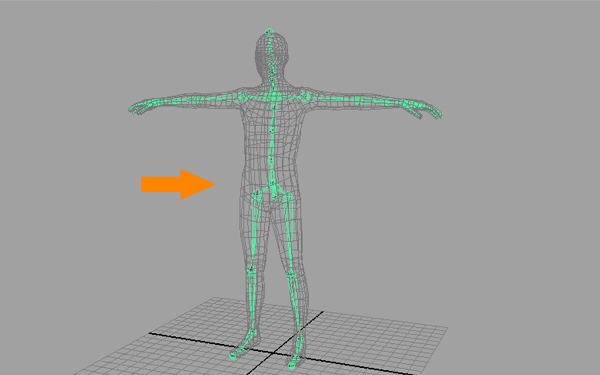
\includegraphics[width=\textwidth]{human_rig}
		\end{column}
		\begin{column}{0.58\textwidth}
			\begin{itemize}
				\pause\item A \textbf{skeleton} is composed of \textbf{bones}
				\pause\item Arranged in a \textbf{hierarchy}
				\pause\item Each bone is essentially just a \textbf{transformation}
					\begin{itemize}
						\pause\item Usually just rotation around a pivot point
						\pause\item 3D modelling software often represents bones as lines from parent bone to child bone
					\end{itemize}
			\end{itemize}
		\end{column}
	\end{columns}
\end{frame}

\begin{frame}{Keyframe animation}
	\begin{itemize}
		\pause\item Most basic form of skeletal animation: specify bone transformations for each frame of animation
		\pause\item ... or just for \textbf{keyframes} and interpolate between them
		\pause\item Keyframes set up by an animator, through motion capture, or a combination of the two
		\pause\item More advanced: can \textbf{blend} animations
			\begin{itemize}
				\pause\item E.g.\ blend between walking and running
				\pause\item E.g.\ bottom half plays ``walk'' animation, top half plays ``fire weapon'' animation
			\end{itemize}
	\end{itemize}
\end{frame}

\begin{frame}{Forward kinematics (FK)}
	\begin{columns}
		\begin{column}{0.4\textwidth}
			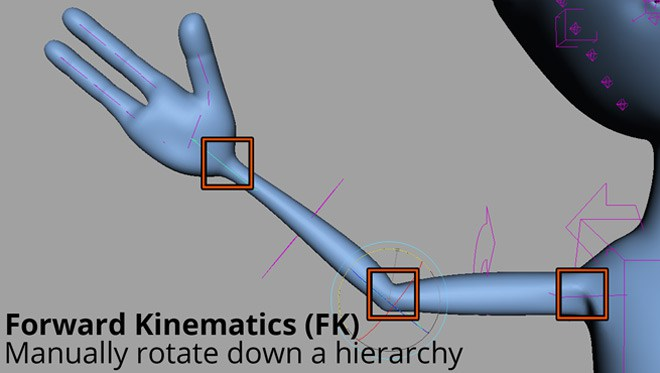
\includegraphics[width=\textwidth]{forward_kinematics}
		\end{column}
		\begin{column}{0.58\textwidth}
			\begin{itemize}
				\pause\item Bone transformations are set \textbf{explicitly}
				\pause\item Children are affected by parent transformations,
					e.g.\ if upper arm rotates, lower arm rotates with it
			\end{itemize}
		\end{column}
	\end{columns}
\end{frame}

\begin{frame}{Inverse kinematics (IK)}
	\begin{columns}
		\begin{column}{0.4\textwidth}
			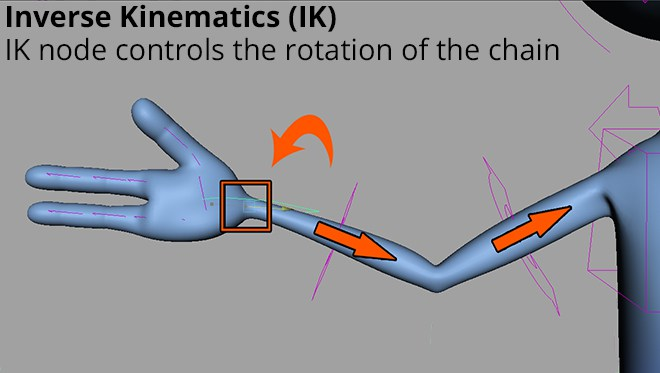
\includegraphics[width=\textwidth]{inverse_kinematics}
		\end{column}
		\begin{column}{0.58\textwidth}
			\begin{itemize}
				\pause\item Bone transformations are calculated to reach a \textbf{target}
				\pause\item E.g.\ we want character's hand to touch an object; IK calculates rotations of upper and lower arm to achieve this
					subject to constraints
			\end{itemize}
		\end{column}
	\end{columns}
\end{frame}

\begin{frame}{The most common use for IK}
	\begin{center}
		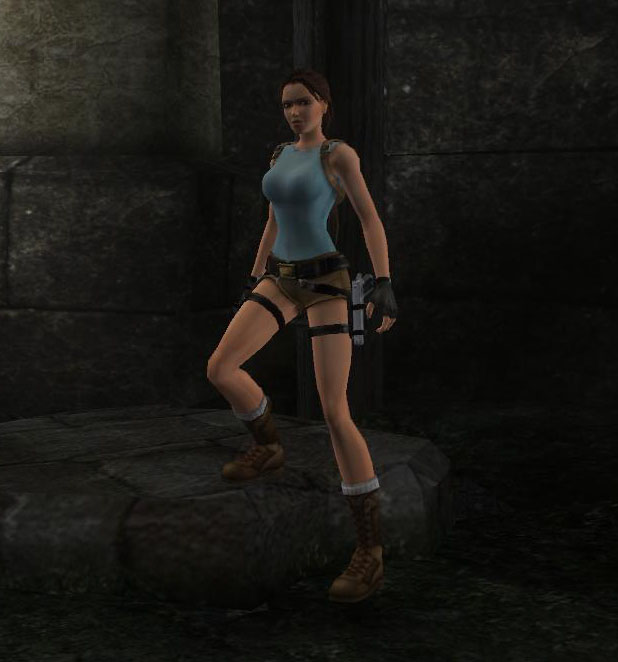
\includegraphics[height=0.4\textheight]{ik_feet3} \quad
		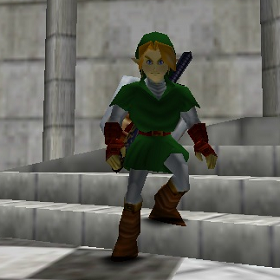
\includegraphics[height=0.4\textheight]{ik_feet2}
		
		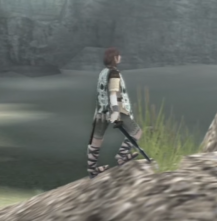
\includegraphics[height=0.4\textheight]{ik_feet4} \quad
		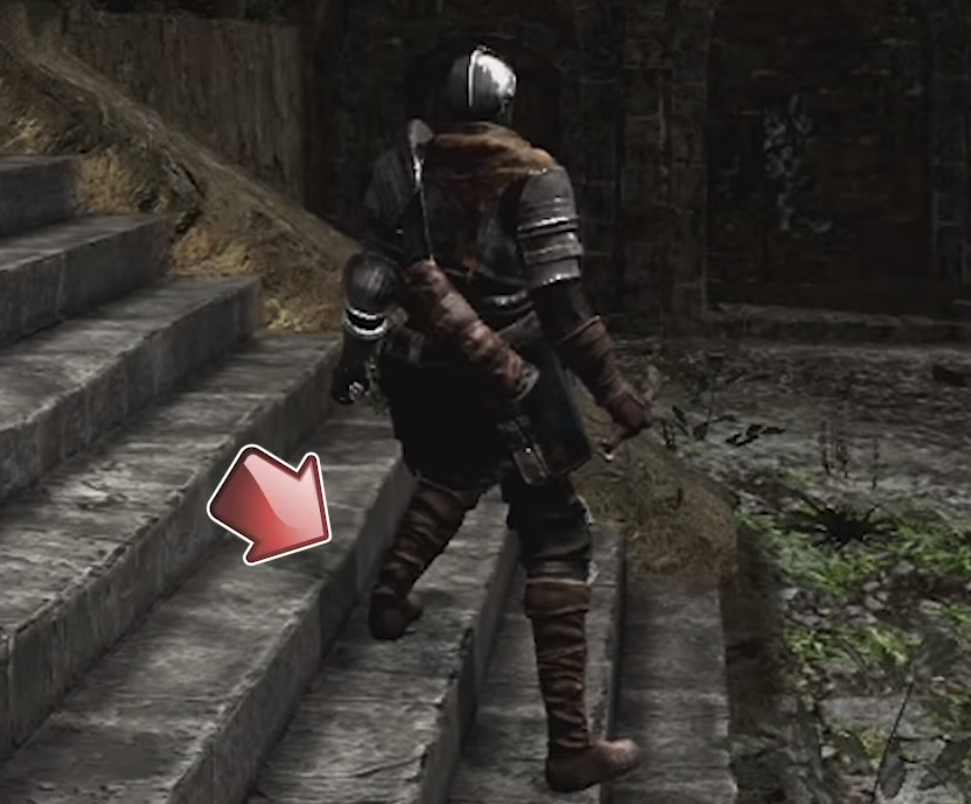
\includegraphics[height=0.4\textheight]{ik_feet}
	\end{center}
\end{frame}

\begin{frame}{Ragdolls}
	\begin{columns}
		\begin{column}{0.4\textwidth}
			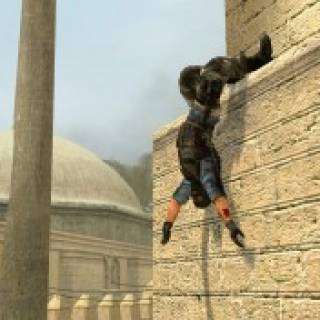
\includegraphics[width=\textwidth]{ragdoll}
		\end{column}
		\begin{column}{0.58\textwidth}
			\begin{itemize}
				\pause\item Attach a \textbf{rigid body} to each bone and run a \textbf{physics simulation}
				\pause\item Often used for death animations
				\pause\item Many games mix and blend some or all of keyframe animation, IK, and physics simulation
			\end{itemize}
		\end{column}
	\end{columns}
\end{frame}

\begin{frame}{Skinning}
	\begin{itemize}
		\pause\item The character is animated by changing the bone transformations
		\pause\item \textbf{Skinning} is the process of applying these transformations to the vertices of the model
		\pause\item Generally handled by a \textbf{vertex shader}
		\pause\item Uses \textbf{bone weights} to specify how much each vertex is affected by each bone's transformation
	\end{itemize}
\end{frame}

\begin{frame}{Bone weights}
	\begin{columns}
		\begin{column}{0.4\textwidth}
			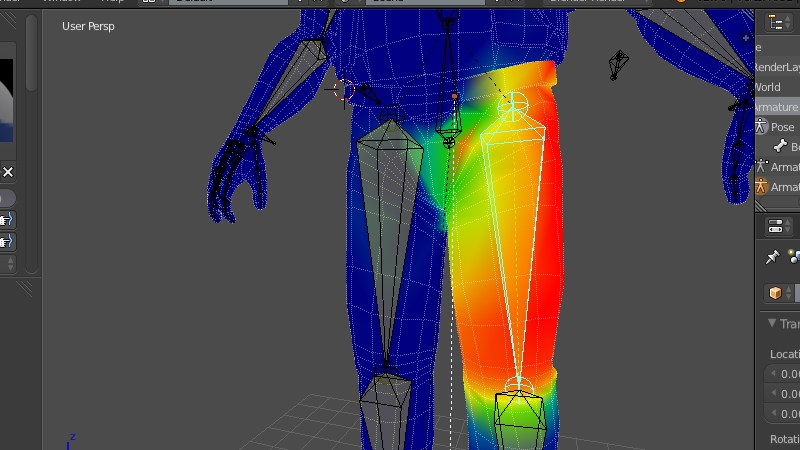
\includegraphics[width=\textwidth]{bone_weights}
		\end{column}
		\begin{column}{0.58\textwidth}
			\begin{itemize}
				\pause\item Each vertex in the model has a list of \textbf{bone weights}
				\pause\item Usually ``painted'' onto the model by the 3D artist
				\pause\item Vertex position is calculated as a weighted average of joint transforms
			\end{itemize}
		\end{column}
	\end{columns}
\end{frame}

\begin{frame}{Secondary effects}
	\begin{itemize}
		\pause\item Additional movement that occurs as a result of the skeletal animation
		\pause\item For example: swinging clothes or hair, jiggle of body parts, skin sliding over bones
		\pause\item Can be \textbf{simulated} using a variety of techniques, though this is often expensive even for simplified methods
		\pause\item A popular approach is to use \textbf{morph targets} (aka \textbf{blend shapes})
	\end{itemize}
\end{frame}

\begin{frame}{Morph targets}
	\begin{itemize}
		\pause\item Take two (or more) \textbf{topologically identical} meshes (i.e. the same vertices in the same order)
		\pause\item Deform each mesh to represent a different \textbf{target}, e.g. happy, sad, angry, neutral
		\pause\item Create effects by \textbf{interpolating} the vertex positions to blend between the targets
	\end{itemize}
	\begin{figure}[h!]
		\pause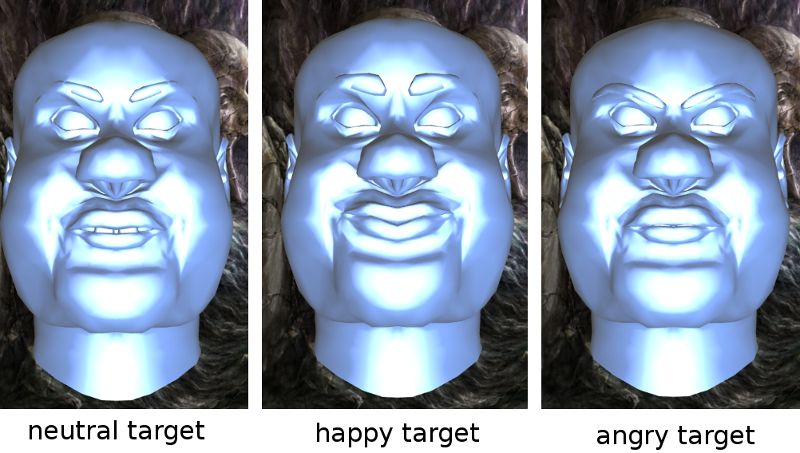
\includegraphics[width=0.4\textwidth]{morph_targets}
		\caption*{Image source: \url{https://antongerdelan.net/opengl/blend_shapes.html}}
	\end{figure}
\end{frame}
